

\begin{frame}{Benchmark Setting}

  \begin{block}{Scope for Portability Study}
    \begin{itemize}
     \item Vector and matrix-vector operations (BLAS levels 1 and 2)
     \item Limited by memory bandwidth
     %\item Matrix-matrix-multiplication (only briefly today)
    \end{itemize}
  \end{block}

  %\pause
  \begin{block}{Key Question (Memory-Bandwidth-Limited Kernels)}
    \begin{center} \color{red} \LARGE
     Good performance of complicated kernels \\
     by optimizing the simplest kernel?
    \end{center}
  \end{block}

\end{frame}


%% Copy kernel:
\begin{frame}[fragile]{Benchmark Setting}
  \begin{block}{Vector Assignment (Copy) Kernel}
    \begin{itemize}
     \item $x \Leftarrow y$ for (large) vectors $x$, $y$
    \end{itemize}
  \end{block}

  \begin{center} \vspace*{0.30cm} 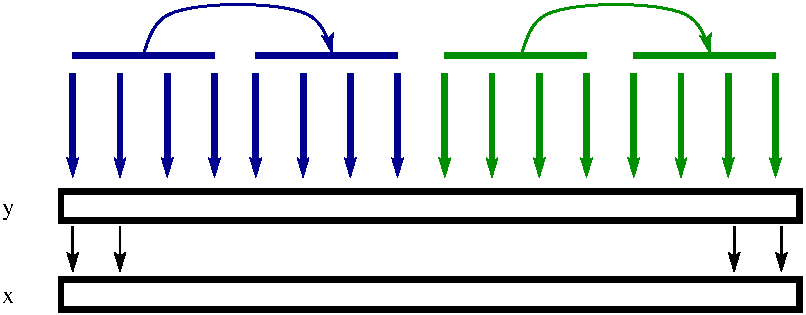
\includegraphics[width=0.8\textwidth]{figures/copy-kernel-cpu-full} \end{center}
  
  \begin{block}{Parameters (1900 variations) }
   \begin{itemize}
     \item \texttt{for (size\_t i = group\_start + get\_local\_id(0);}
     \item \texttt{\ \ \ \ \ i < group\_end; i+= get\_local\_size(0)) }
     \item \texttt{\ \  x[i] = y[i];}
   \end{itemize}
  \end{block}
\end{frame}


%% 
\begin{frame}{Benchmark Setting}

  \begin{block}{Operations}
   \begin{itemize}
    \item Vector copy, vector addition, inner product
    \item Matrix-vector product
   \end{itemize}
  \end{block}

  \begin{center} 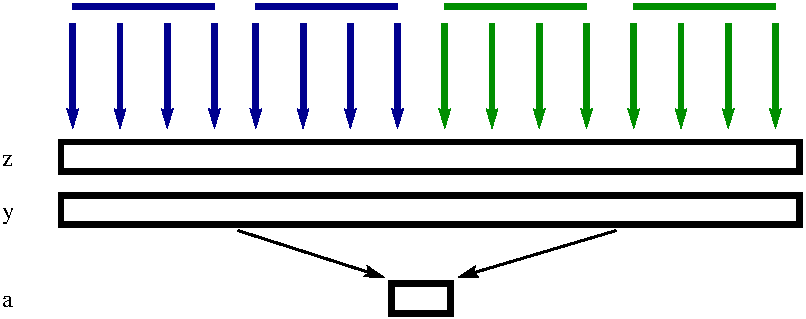
\includegraphics[width=0.8\textwidth]{figures/inner-product-kernel} \end{center}

  \begin{block}{Devices}
   \begin{itemize}
    \item AMD: A10-5800 APU, HD 5850 GPU
    \item INTEL: Dual Socket Xeon E5-2670, Xeon Phi
    \item NVIDIA: GTX 285, Tesla K20m
   \end{itemize}
  \end{block}
  
\end{frame}
